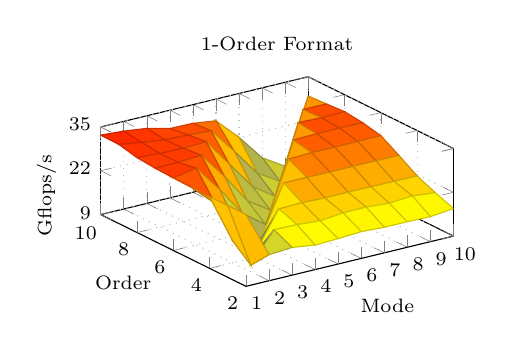
\begin{tikzpicture}
\begin{axis}[height=0.35\textwidth,width=0.5\textwidth,style={font=\scriptsize},grid=major,grid style={dotted},align=center,xlabel={Mode},ylabel={Order},zlabel={Gflops/s},title={$1$-Order Format}, xtick={1,2,3,4,5,6,7,8,9,10},xticklabels={1,2,3,4,5,6,7,8,9,10}, ytick={2,4,6,8,10}, yticklabels={2,4,6,8,10}, point meta max=35, point meta min=9, zmin=9, zmax=35, ztick={9,22,35},zticklabels={9,22,35}, view={-35}{45}, xlabel style={yshift=2mm}, ylabel style={yshift=4mm}, zlabel style={yshift=-1mm,xshift=-4mm}]
\addplot3[surf] %,colormap = {whiteblack}{color(0cm)=(white);color(0.4cm) = (darkgray)}
coordinates{
(1.000,2.000,30.353) (1.000,3.000,30.312) (1.000,4.000,30.265) (1.000,5.000,30.361) (1.000,6.000,30.506) (1.000,7.000,30.751) (1.000,8.000,31.224) (1.000,9.000,32.470) (1.000,10.000,32.590) 

(2.000,2.000,16.748) (2.000,3.000,10.971) (2.000,4.000,15.539) (2.000,5.000,24.166) (2.000,6.000,31.744) (2.000,7.000,30.820) (2.000,8.000,30.771) (2.000,9.000,31.394) (2.000,10.000,32.110) 

(3.000,2.000,17.232) (3.000,3.000,19.809) (3.000,4.000,10.343) (3.000,5.000,15.135) (3.000,6.000,23.893) (3.000,7.000,31.252) (3.000,8.000,30.718) (3.000,9.000,30.505) (3.000,10.000,31.268) 

(4.000,2.000,16.270) (4.000,3.000,19.656) (4.000,4.000,21.676) (4.000,5.000,9.964) (4.000,6.000,14.975) (4.000,7.000,23.383) (4.000,8.000,30.969) (4.000,9.000,30.341) (4.000,10.000,29.576) 

(5.000,2.000,16.531) (5.000,3.000,19.141) (5.000,4.000,21.867) (5.000,5.000,25.058) (5.000,6.000,10.071) (5.000,7.000,14.425) (5.000,8.000,22.690) (5.000,9.000,29.897) (5.000,10.000,29.463) 

(6.000,2.000,16.960) (6.000,3.000,19.837) (6.000,4.000,21.600) (6.000,5.000,25.039) (6.000,6.000,27.817) (6.000,7.000,9.995) (6.000,8.000,14.451) (6.000,9.000,22.192) (6.000,10.000,28.544) 

(7.000,2.000,16.580) (7.000,3.000,19.918) (7.000,4.000,21.691) (7.000,5.000,24.989) (7.000,6.000,28.077) (7.000,7.000,29.165) (7.000,8.000,9.692) (7.000,9.000,14.040) (7.000,10.000,21.983) 

(8.000,2.000,16.580) (8.000,3.000,19.375) (8.000,4.000,21.619) (8.000,5.000,25.026) (8.000,6.000,28.052) (8.000,7.000,29.365) (8.000,8.000,30.029) (8.000,9.000,9.851) (8.000,10.000,14.291) 

(9.000,2.000,16.414) (9.000,3.000,19.905) (9.000,4.000,21.575) (9.000,5.000,25.011) (9.000,6.000,28.093) (9.000,7.000,29.394) (9.000,8.000,29.785) (9.000,9.000,29.598) (9.000,10.000,10.064) 

(10.000,2.000,17.212) (10.000,3.000,19.196) (10.000,4.000,21.529) (10.000,5.000,24.939) (10.000,6.000,28.175) (10.000,7.000,29.346) (10.000,8.000,29.977) (10.000,9.000,29.587) (10.000,10.000,29.286) 

};
\end{axis}
\end{tikzpicture}
\begin{comment}
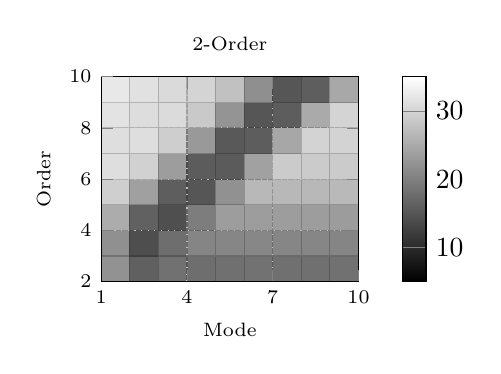
\begin{tikzpicture}
\begin{axis}[width=0.40\textwidth,style={font=\scriptsize},grid=major,grid style={dotted},align=center,xlabel={Mode},ylabel={Order},zlabel={Gflops/s},title={2-Order}, xtick={1,4,7,10},xticklabels={1,4,7,10}, ytick={2,4,6,8,10}, yticklabels={2,4,6,8,10}, point meta max=35, point meta min=5, ztick={5,15,25,35},zticklabels={5,15,25,35}, view={0}{90}, colorbar,colormap/blackwhite, colorbar style={width=0.3cm}]
\addplot3[surf] %  colormap/blackwhite ,shader=faceted interp, colormap = {whiteblack}{color(0cm)=(white);color(0.4cm) = (darkgray)}
coordinates{(1.000,2.000,30.353) (1.000,3.000,30.312) (1.000,4.000,30.265) (1.000,5.000,30.361) (1.000,6.000,30.506) (1.000,7.000,30.751) (1.000,8.000,31.224) (1.000,9.000,32.470) (1.000,10.000,32.590) 

(2.000,2.000,16.748) (2.000,3.000,10.971) (2.000,4.000,15.539) (2.000,5.000,24.166) (2.000,6.000,31.744) (2.000,7.000,30.820) (2.000,8.000,30.771) (2.000,9.000,31.394) (2.000,10.000,32.110) 

(3.000,2.000,17.232) (3.000,3.000,19.809) (3.000,4.000,10.343) (3.000,5.000,15.135) (3.000,6.000,23.893) (3.000,7.000,31.252) (3.000,8.000,30.718) (3.000,9.000,30.505) (3.000,10.000,31.268) 

(4.000,2.000,16.270) (4.000,3.000,19.656) (4.000,4.000,21.676) (4.000,5.000,9.964) (4.000,6.000,14.975) (4.000,7.000,23.383) (4.000,8.000,30.969) (4.000,9.000,30.341) (4.000,10.000,29.576) 

(5.000,2.000,16.531) (5.000,3.000,19.141) (5.000,4.000,21.867) (5.000,5.000,25.058) (5.000,6.000,10.071) (5.000,7.000,14.425) (5.000,8.000,22.690) (5.000,9.000,29.897) (5.000,10.000,29.463) 

(6.000,2.000,16.960) (6.000,3.000,19.837) (6.000,4.000,21.600) (6.000,5.000,25.039) (6.000,6.000,27.817) (6.000,7.000,9.995) (6.000,8.000,14.451) (6.000,9.000,22.192) (6.000,10.000,28.544) 

(7.000,2.000,16.580) (7.000,3.000,19.918) (7.000,4.000,21.691) (7.000,5.000,24.989) (7.000,6.000,28.077) (7.000,7.000,29.165) (7.000,8.000,9.692) (7.000,9.000,14.040) (7.000,10.000,21.983) 

(8.000,2.000,16.580) (8.000,3.000,19.375) (8.000,4.000,21.619) (8.000,5.000,25.026) (8.000,6.000,28.052) (8.000,7.000,29.365) (8.000,8.000,30.029) (8.000,9.000,9.851) (8.000,10.000,14.291) 

(9.000,2.000,16.414) (9.000,3.000,19.905) (9.000,4.000,21.575) (9.000,5.000,25.011) (9.000,6.000,28.093) (9.000,7.000,29.394) (9.000,8.000,29.785) (9.000,9.000,29.598) (9.000,10.000,10.064) 

(10.000,2.000,17.212) (10.000,3.000,19.196) (10.000,4.000,21.529) (10.000,5.000,24.939) (10.000,6.000,28.175) (10.000,7.000,29.346) (10.000,8.000,29.977) (10.000,9.000,29.587) (10.000,10.000,29.286) 

};
\end{axis}
\end{tikzpicture}
\end{comment}
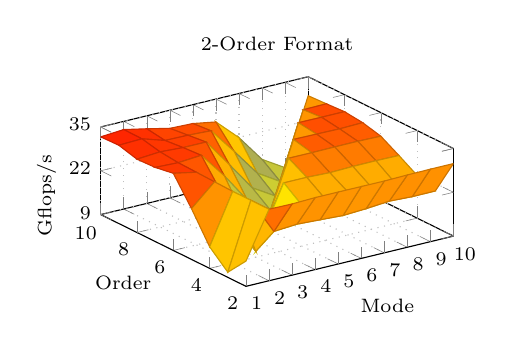
\begin{tikzpicture}
\begin{axis}[height=0.35\textwidth,width=0.5\textwidth,style={font=\scriptsize},grid=major,grid style={dotted},align=center,xlabel={Mode},ylabel={Order},zlabel={Gflops/s},title={$2$-Order Format}, xtick={1,2,3,4,5,6,7,8,9,10},xticklabels={1,2,3,4,5,6,7,8,9,10}, ytick={2,4,6,8,10}, yticklabels={2,4,6,8,10}, point meta max=35, point meta min=9, zmin=9, zmax=35, ztick={9,22,35},zticklabels={9,22,35}, view={-35}{45}, xlabel style={yshift=2mm}, ylabel style={yshift=4mm}, zlabel style={yshift=-1mm,xshift=-4mm}]
\addplot3[surf] %,colormap/blackwhite ,shader=faceted interp, colormap = {whiteblack}{color(0cm)=(white);color(0.4cm) = (darkgray)}  
coordinates{
(1.000,2.000,16.487) (1.000,3.000,10.523) (1.000,4.000,15.395) (1.000,5.000,24.073) (1.000,6.000,31.895) (1.000,7.000,30.984) (1.000,8.000,30.758) (1.000,9.000,32.238) (1.000,10.000,32.059) 

(2.000,2.000,30.222) (2.000,3.000,30.212) (2.000,4.000,30.186) (2.000,5.000,30.372) (2.000,6.000,30.553) (2.000,7.000,30.716) (2.000,8.000,31.277) (2.000,9.000,32.485) (2.000,10.000,32.573) 

(3.000,2.000,30.131) (3.000,3.000,19.318) (3.000,4.000,10.731) (3.000,5.000,15.162) (3.000,6.000,23.937) (3.000,7.000,31.261) (3.000,8.000,30.887) (3.000,9.000,30.344) (3.000,10.000,31.150) 

(4.000,2.000,30.361) (4.000,3.000,19.814) (4.000,4.000,21.447) (4.000,5.000,10.324) (4.000,6.000,14.858) (4.000,7.000,23.518) (4.000,8.000,30.873) (4.000,9.000,30.238) (4.000,10.000,29.623) 

(5.000,2.000,30.360) (5.000,3.000,19.462) (5.000,4.000,21.109) (5.000,5.000,25.090) (5.000,6.000,9.819) (5.000,7.000,14.619) (5.000,8.000,22.566) (5.000,9.000,29.901) (5.000,10.000,29.393) 

(6.000,2.000,30.335) (6.000,3.000,19.079) (6.000,4.000,21.407) (6.000,5.000,25.074) (6.000,6.000,28.086) (6.000,7.000,9.972) (6.000,8.000,13.973) (6.000,9.000,22.128) (6.000,10.000,28.208) 

(7.000,2.000,30.310) (7.000,3.000,19.451) (7.000,4.000,21.691) (7.000,5.000,24.793) (7.000,6.000,28.064) (7.000,7.000,29.357) (7.000,8.000,9.892) (7.000,9.000,14.045) (7.000,10.000,21.885) 

(8.000,2.000,30.456) (8.000,3.000,20.016) (8.000,4.000,21.611) (8.000,5.000,24.992) (8.000,6.000,28.120) (8.000,7.000,29.268) (8.000,8.000,30.003) (8.000,9.000,9.867) (8.000,10.000,13.789) 

(9.000,2.000,30.526) (9.000,3.000,19.705) (9.000,4.000,21.412) (9.000,5.000,25.037) (9.000,6.000,28.145) (9.000,7.000,29.169) (9.000,8.000,29.956) (9.000,9.000,29.528) (9.000,10.000,9.665) 

(10.000,2.000,30.524) (10.000,3.000,19.731) (10.000,4.000,21.676) (10.000,5.000,24.930) (10.000,6.000,27.992) (10.000,7.000,29.354) (10.000,8.000,29.951) (10.000,9.000,29.632) (10.000,10.000,29.359) 

};
\end{axis}
\end{tikzpicture}
\begin{comment}
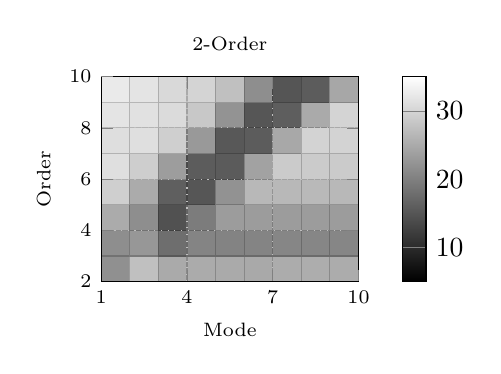
\begin{tikzpicture}
%\begin{axis}[width=0.45\textwidth,style={font=\scriptsize},grid=major,grid style={dotted},align=center,xlabel={Contractionmode},xlabel near ticks,ylabel={Tensorrank},zlabel={Gflops/s},title={2-Order}, xtick={1,4,7,10},xticklabels={1,4,7,10}, ytick={2,4,6,8,10}, yticklabels={2,4,6,8,10}, ztick={5,15,25,35},zticklabels={5,15,25,35}, view={-45}{45}]
%\addplot3[surf,shader=faceted interp, colormap = {whiteblack}{color(0cm)=(white);color(0.4cm) = (darkgray)}] %  colormap/blackwhite
\begin{axis}[width=0.40\textwidth,style={font=\scriptsize},grid=major,grid style={dotted},align=center,xlabel={Mode},ylabel={Order},zlabel={Gflops/s},title={2-Order}, xtick={1,4,7,10},xticklabels={1,4,7,10}, ytick={2,4,6,8,10}, yticklabels={2,4,6,8,10}, point meta max=35, point meta min=5, ztick={5,15,25,35},zticklabels={5,15,25,35}, view={0}{90}, colorbar,colormap/blackwhite, colorbar style={width=0.3cm}]
\addplot3[surf] %  ,colormap/blackwhite ,shader=faceted interp, colormap = {whiteblack}{color(0cm)=(white);color(0.4cm) = (darkgray)}
coordinates{(1.000,2.000,16.487) (1.000,3.000,10.523) (1.000,4.000,15.395) (1.000,5.000,24.073) (1.000,6.000,31.895) (1.000,7.000,30.984) (1.000,8.000,30.758) (1.000,9.000,32.238) (1.000,10.000,32.059) 

(2.000,2.000,30.222) (2.000,3.000,30.212) (2.000,4.000,30.186) (2.000,5.000,30.372) (2.000,6.000,30.553) (2.000,7.000,30.716) (2.000,8.000,31.277) (2.000,9.000,32.485) (2.000,10.000,32.573) 

(3.000,2.000,30.131) (3.000,3.000,19.318) (3.000,4.000,10.731) (3.000,5.000,15.162) (3.000,6.000,23.937) (3.000,7.000,31.261) (3.000,8.000,30.887) (3.000,9.000,30.344) (3.000,10.000,31.150) 

(4.000,2.000,30.361) (4.000,3.000,19.814) (4.000,4.000,21.447) (4.000,5.000,10.324) (4.000,6.000,14.858) (4.000,7.000,23.518) (4.000,8.000,30.873) (4.000,9.000,30.238) (4.000,10.000,29.623) 

(5.000,2.000,30.360) (5.000,3.000,19.462) (5.000,4.000,21.109) (5.000,5.000,25.090) (5.000,6.000,9.819) (5.000,7.000,14.619) (5.000,8.000,22.566) (5.000,9.000,29.901) (5.000,10.000,29.393) 

(6.000,2.000,30.335) (6.000,3.000,19.079) (6.000,4.000,21.407) (6.000,5.000,25.074) (6.000,6.000,28.086) (6.000,7.000,9.972) (6.000,8.000,13.973) (6.000,9.000,22.128) (6.000,10.000,28.208) 

(7.000,2.000,30.310) (7.000,3.000,19.451) (7.000,4.000,21.691) (7.000,5.000,24.793) (7.000,6.000,28.064) (7.000,7.000,29.357) (7.000,8.000,9.892) (7.000,9.000,14.045) (7.000,10.000,21.885) 

(8.000,2.000,30.456) (8.000,3.000,20.016) (8.000,4.000,21.611) (8.000,5.000,24.992) (8.000,6.000,28.120) (8.000,7.000,29.268) (8.000,8.000,30.003) (8.000,9.000,9.867) (8.000,10.000,13.789) 

(9.000,2.000,30.526) (9.000,3.000,19.705) (9.000,4.000,21.412) (9.000,5.000,25.037) (9.000,6.000,28.145) (9.000,7.000,29.169) (9.000,8.000,29.956) (9.000,9.000,29.528) (9.000,10.000,9.665) 

(10.000,2.000,30.524) (10.000,3.000,19.731) (10.000,4.000,21.676) (10.000,5.000,24.930) (10.000,6.000,27.992) (10.000,7.000,29.354) (10.000,8.000,29.951) (10.000,9.000,29.632) (10.000,10.000,29.359) 

};
\end{axis}
\end{tikzpicture}
\end{comment}


%%%%%%%%%%%%%%%%%%%%%%%%%
%%%%%%%%%%%%%%%%%%%%%%%%%

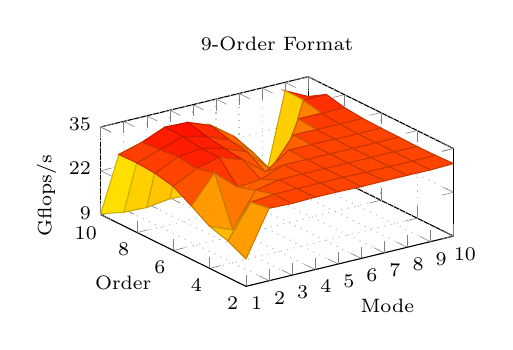
\begin{tikzpicture}
\begin{axis}[height=0.35\textwidth,width=0.5\textwidth,style={font=\scriptsize},grid=major,grid style={dotted},align=center,xlabel={Mode},ylabel={Order},zlabel={Gflops/s},title={$9$-Order Format}, xtick={1,2,3,4,5,6,7,8,9,10},xticklabels={1,2,3,4,5,6,7,8,9,10}, ytick={2,4,6,8,10}, yticklabels={2,4,6,8,10}, point meta max=35, point meta min=9, zmin=9, zmax=35, ztick={9,22,35},zticklabels={9,22,35}, view={-35}{45}, xlabel style={yshift=2mm}, ylabel style={yshift=4mm}, zlabel style={yshift=-1mm,xshift=-4mm}]
\addplot3[surf] %, colormap = {whiteblack}{color(0cm)=(white);color(0.4cm) = (darkgray)}
coordinates{
(1.000,2.000,17.129) (1.000,3.000,19.813) (1.000,4.000,21.480) (1.000,5.000,24.831) (1.000,6.000,28.007) (1.000,7.000,29.212) (1.000,8.000,29.648) (1.000,9.000,29.509) (1.000,10.000,9.204) 

(2.000,2.000,30.515) (2.000,3.000,29.627) (2.000,4.000,18.732) (2.000,5.000,33.044) (2.000,6.000,31.688) (2.000,7.000,32.481) (2.000,8.000,31.983) (2.000,9.000,31.437) (2.000,10.000,8.033) 

(3.000,2.000,30.283) (3.000,3.000,30.326) (3.000,4.000,28.877) (3.000,5.000,27.145) (3.000,6.000,33.324) (3.000,7.000,33.272) (3.000,8.000,34.140) (3.000,9.000,34.297) (3.000,10.000,7.806) 

(4.000,2.000,30.481) (4.000,3.000,30.330) (4.000,4.000,30.260) (4.000,5.000,27.751) (4.000,6.000,31.000) (4.000,7.000,31.675) (4.000,8.000,32.562) (4.000,9.000,34.035) (4.000,10.000,8.720) 

(5.000,2.000,30.460) (5.000,3.000,30.363) (5.000,4.000,30.381) (5.000,5.000,30.380) (5.000,6.000,25.669) (5.000,7.000,28.912) (5.000,8.000,29.837) (5.000,9.000,31.473) (5.000,10.000,8.323) 

(6.000,2.000,30.289) (6.000,3.000,30.392) (6.000,4.000,30.314) (6.000,5.000,30.366) (6.000,6.000,30.487) (6.000,7.000,22.045) (6.000,8.000,24.634) (6.000,9.000,26.550) (6.000,10.000,7.492) 

(7.000,2.000,30.361) (7.000,3.000,30.244) (7.000,4.000,30.325) (7.000,5.000,30.351) (7.000,6.000,30.472) (7.000,7.000,30.667) (7.000,8.000,15.462) (7.000,9.000,17.764) (7.000,10.000,6.490) 

(8.000,2.000,30.368) (8.000,3.000,30.239) (8.000,4.000,30.302) (8.000,5.000,30.322) (8.000,6.000,30.423) (8.000,7.000,30.604) (8.000,8.000,31.118) (8.000,9.000,10.020) (8.000,10.000,3.702) 

(9.000,2.000,30.302) (9.000,3.000,30.263) (9.000,4.000,30.374) (9.000,5.000,30.381) (9.000,6.000,30.290) (9.000,7.000,30.575) (9.000,8.000,31.125) (9.000,9.000,32.377) (9.000,10.000,32.499) 

(10.000,2.000,30.528) (10.000,3.000,30.308) (10.000,4.000,30.248) (10.000,5.000,30.360) (10.000,6.000,30.425) (10.000,7.000,30.623) (10.000,8.000,31.143) (10.000,9.000,32.405) (10.000,10.000,29.128) 

};
\end{axis}
\end{tikzpicture}
\begin{comment}
\begin{tikzpicture}
\begin{axis}[height=0.40\textheight,width=0.40\textwidth,style={font=\footnotesize},grid=major,grid style={dotted},align=center,xlabel={Kontraktionsmodus},ylabel={Tensorstufe},title={TLib-LB-PB1},scaled ticks=false,zticklabel=\pgfmathprintnumber{\tick},zlabel={Durchsatz [Gflops/s]},view={-45}{45}, zlabel={Standardfehler [\%]}]
\addplot3[surf]
coordinates{(1.000,2.000,1.332) (1.000,3.000,2.323) (1.000,4.000,1.343) (1.000,5.000,2.804) (1.000,6.000,2.185) (1.000,7.000,1.776) (1.000,8.000,3.519) (1.000,9.000,1.011) (1.000,10.000,8.378) 

(2.000,2.000,0.982) (2.000,3.000,13.229) (2.000,4.000,9.766) (2.000,5.000,8.786) (2.000,6.000,8.573) (2.000,7.000,7.481) (2.000,8.000,3.903) (2.000,9.000,1.505) (2.000,10.000,10.030) 

(3.000,2.000,3.028) (3.000,3.000,2.194) (3.000,4.000,17.840) (3.000,5.000,17.637) (3.000,6.000,15.227) (3.000,7.000,14.487) (3.000,8.000,8.447) (3.000,9.000,1.892) (3.000,10.000,8.646) 

(4.000,2.000,1.246) (4.000,3.000,2.092) (4.000,4.000,3.240) (4.000,5.000,23.698) (4.000,6.000,23.113) (4.000,7.000,23.313) (4.000,8.000,17.243) (4.000,9.000,7.588) (4.000,10.000,7.767) 

(5.000,2.000,1.784) (5.000,3.000,2.086) (5.000,4.000,2.754) (5.000,5.000,3.265) (5.000,6.000,30.565) (5.000,7.000,31.968) (5.000,8.000,27.869) (5.000,9.000,18.713) (5.000,10.000,9.655) 

(6.000,2.000,3.050) (6.000,3.000,1.930) (6.000,4.000,3.008) (6.000,5.000,3.280) (6.000,6.000,3.699) (6.000,7.000,41.861) (6.000,8.000,40.665) (6.000,9.000,33.483) (6.000,10.000,9.785) 

(7.000,2.000,1.125) (7.000,3.000,2.431) (7.000,4.000,2.940) (7.000,5.000,3.223) (7.000,6.000,3.827) (7.000,7.000,4.337) (7.000,8.000,49.526) (7.000,9.000,47.835) (7.000,10.000,12.546) 

(8.000,2.000,1.147) (8.000,3.000,2.508) (8.000,4.000,3.005) (8.000,5.000,2.770) (8.000,6.000,3.539) (8.000,7.000,3.996) (8.000,8.000,4.144) (8.000,9.000,58.162) (8.000,10.000,13.963) 

(9.000,2.000,3.252) (9.000,3.000,2.411) (9.000,4.000,2.776) (9.000,5.000,3.117) (9.000,6.000,5.433) (9.000,7.000,4.170) (9.000,8.000,4.123) (9.000,9.000,0.672) (9.000,10.000,0.797) 

(10.000,2.000,1.467) (10.000,3.000,2.076) (10.000,4.000,3.202) (10.000,5.000,3.244) (10.000,6.000,3.931) (10.000,7.000,4.243) (10.000,8.000,4.159) (10.000,9.000,1.011) (10.000,10.000,2.226) 

};\end{axis}
\end{tikzpicture}
\end{comment}
\begin{comment}
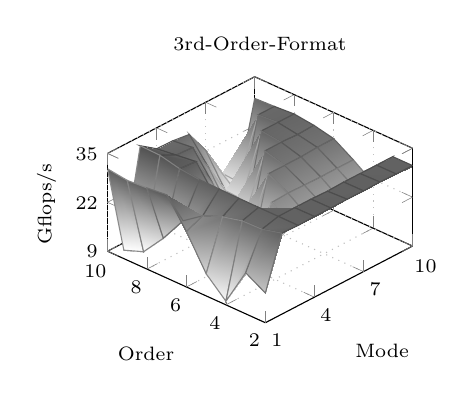
\begin{tikzpicture}
\begin{axis}[width=0.45\textwidth,style={font=\scriptsize},grid=major,grid style={dotted},align=center,xlabel={Mode},ylabel={Order},zlabel={Gflops/s},title={3rd-Order-Format}, xtick={1,4,7,10},xticklabels={1,4,7,10}, ytick={2,4,6,8,10}, yticklabels={2,4,6,8,10}, point meta max=35, point meta min=9, zmin=9, zmax=35, ztick={9,22,35},zticklabels={9,22,35}, view={-47}{47}, ] %
\addplot3[surf,shader=faceted interp, colormap = {whiteblack}{color(0cm)=(white);color(0.4cm) = (darkgray)}] %  colormap/blackwhite
coordinates{
(1.000,2.000,16.903) (1.000,3.000,19.899) (1.000,4.000,9.972) (1.000,5.000,14.884) (1.000,6.000,23.730) (1.000,7.000,31.140) (1.000,8.000,30.576) (1.000,9.000,30.207) (1.000,10.000,30.915) 

(2.000,2.000,30.562) (2.000,3.000,29.215) (2.000,4.000,29.073) (2.000,5.000,27.765) (2.000,6.000,25.665) (2.000,7.000,21.957) (2.000,8.000,14.935) (2.000,9.000,8.976) (2.000,10.000,7.009) 

(3.000,2.000,30.335) (3.000,3.000,30.356) (3.000,4.000,30.356) (3.000,5.000,30.404) (3.000,6.000,30.503) (3.000,7.000,30.627) (3.000,8.000,31.162) (3.000,9.000,32.369) (3.000,10.000,32.511) 

(4.000,2.000,30.443) (4.000,3.000,30.413) (4.000,4.000,21.309) (4.000,5.000,10.070) (4.000,6.000,14.819) (4.000,7.000,23.495) (4.000,8.000,30.785) (4.000,9.000,30.121) (4.000,10.000,29.447) 

(5.000,2.000,30.441) (5.000,3.000,30.415) (5.000,4.000,21.189) (5.000,5.000,24.741) (5.000,6.000,9.830) (5.000,7.000,14.105) (5.000,8.000,22.859) (5.000,9.000,29.890) (5.000,10.000,29.293) 

(6.000,2.000,30.501) (6.000,3.000,30.264) (6.000,4.000,21.327) (6.000,5.000,24.995) (6.000,6.000,27.759) (6.000,7.000,9.373) (6.000,8.000,13.735) (6.000,9.000,22.080) (6.000,10.000,28.726) 

(7.000,2.000,30.463) (7.000,3.000,30.424) (7.000,4.000,21.552) (7.000,5.000,24.845) (7.000,6.000,27.708) (7.000,7.000,29.197) (7.000,8.000,9.455) (7.000,9.000,13.912) (7.000,10.000,22.226) 

(8.000,2.000,30.559) (8.000,3.000,30.409) (8.000,4.000,21.183) (8.000,5.000,24.771) (8.000,6.000,27.728) (8.000,7.000,29.236) (8.000,8.000,29.881) (8.000,9.000,9.399) (8.000,10.000,13.882) 

(9.000,2.000,30.413) (9.000,3.000,30.383) (9.000,4.000,21.371) (9.000,5.000,24.801) (9.000,6.000,27.975) (9.000,7.000,29.032) (9.000,8.000,29.869) (9.000,9.000,29.502) (9.000,10.000,9.277) 

(10.000,2.000,30.391) (10.000,3.000,30.378) (10.000,4.000,21.091) (10.000,5.000,24.776) (10.000,6.000,28.059) (10.000,7.000,29.208) (10.000,8.000,29.848) (10.000,9.000,29.484) (10.000,10.000,29.241) 

};
\end{axis}
\end{tikzpicture}
\end{comment}
\begin{comment}
\begin{tikzpicture}
\begin{axis}[height=0.40\textheight,width=0.40\textwidth,style={font=\footnotesize},grid=major,grid style={dotted},align=center,xlabel={Kontraktionsmodus},ylabel={Tensorstufe},title={TLib-LB-PB2},scaled ticks=false,zticklabel=\pgfmathprintnumber{\tick},zlabel={Durchsatz [Gflops/s]},view={-45}{45}, zlabel={Standardfehler [\%]}]
\addplot3[surf]
coordinates{(1.000,2.000,1.307) (1.000,3.000,1.302) (1.000,4.000,10.940) (1.000,5.000,4.791) (1.000,6.000,2.662) (1.000,7.000,1.372) (1.000,8.000,1.192) (1.000,9.000,1.793) (1.000,10.000,1.223) 

(2.000,2.000,1.359) (2.000,3.000,14.470) (2.000,4.000,18.614) (2.000,5.000,23.954) (2.000,6.000,30.664) (2.000,7.000,42.176) (2.000,8.000,49.976) (2.000,9.000,48.495) (2.000,10.000,72.280) 

(3.000,2.000,1.730) (3.000,3.000,2.233) (3.000,4.000,2.992) (3.000,5.000,3.202) (3.000,6.000,3.692) (3.000,7.000,4.356) (3.000,8.000,4.346) (3.000,9.000,1.336) (3.000,10.000,0.967) 

(4.000,2.000,1.249) (4.000,3.000,2.217) (4.000,4.000,1.868) (4.000,5.000,10.989) (4.000,6.000,5.915) (4.000,7.000,1.652) (4.000,8.000,1.266) (4.000,9.000,1.297) (4.000,10.000,1.679) 

(5.000,2.000,1.654) (5.000,3.000,2.156) (5.000,4.000,2.024) (5.000,5.000,2.917) (5.000,6.000,9.904) (5.000,7.000,6.006) (5.000,8.000,2.559) (5.000,9.000,0.933) (5.000,10.000,1.096) 

(6.000,2.000,1.519) (6.000,3.000,2.374) (6.000,4.000,1.717) (6.000,5.000,2.551) (6.000,6.000,2.491) (6.000,7.000,11.882) (6.000,8.000,6.486) (6.000,9.000,2.339) (6.000,10.000,2.331) 

(7.000,2.000,1.545) (7.000,3.000,2.096) (7.000,4.000,1.423) (7.000,5.000,2.617) (7.000,6.000,2.637) (7.000,7.000,1.911) (7.000,8.000,11.610) (7.000,9.000,5.473) (7.000,10.000,2.849) 

(8.000,2.000,1.677) (8.000,3.000,2.111) (8.000,4.000,1.871) (8.000,5.000,2.775) (8.000,6.000,2.158) (8.000,7.000,1.943) (8.000,8.000,1.400) (8.000,9.000,10.778) (8.000,10.000,5.460) 

(9.000,2.000,1.534) (9.000,3.000,2.010) (9.000,4.000,1.628) (9.000,5.000,2.494) (9.000,6.000,2.310) (9.000,7.000,2.047) (9.000,8.000,1.370) (9.000,9.000,1.302) (9.000,10.000,10.568) 

(10.000,2.000,1.603) (10.000,3.000,2.075) (10.000,4.000,1.484) (10.000,5.000,2.817) (10.000,6.000,2.233) (10.000,7.000,1.943) (10.000,8.000,1.591) (10.000,9.000,1.081) (10.000,10.000,0.938) 

};\end{axis}
\end{tikzpicture}
\end{comment}
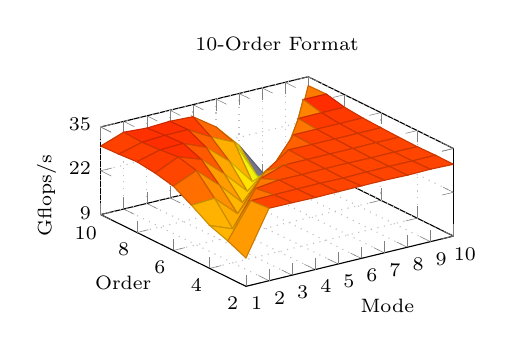
\begin{tikzpicture}
\begin{axis}[height=0.35\textwidth, width=0.5\textwidth,,style={font=\scriptsize},grid=major,grid style={dotted}, align=center, xlabel={Mode}, ylabel={Order}, zlabel={Gflops/s},title={$10$-Order Format}, xtick={1,4,7,10}, xtick={1,2,3,4,5,6,7,8,9,10},xticklabels={1,2,3,4,5,6,7,8,9,10}, ytick={2,4,6,8,10}, yticklabels={2,4,6,8,10}, point meta max=35, point meta min=9, zmin=9, zmax=35, ztick={9,22,35},zticklabels={9,22,35}, view={-35}{45}, xlabel style={yshift=2mm}, ylabel style={yshift=4mm}, zlabel style={yshift=-1mm,xshift=-4mm}]
\addplot3[surf] %, colormap = {whiteblack}{color(0cm)=(white);color(0.4cm) = (darkgray)}
coordinates{
(1.000,2.000,17.409) (1.000,3.000,19.812) (1.000,4.000,21.745) (1.000,5.000,25.078) (1.000,6.000,28.085) (1.000,7.000,29.298) (1.000,8.000,29.987) (1.000,9.000,29.593) (1.000,10.000,29.331) 

(2.000,2.000,30.526) (2.000,3.000,30.078) (2.000,4.000,19.075) (2.000,5.000,25.485) (2.000,6.000,31.053) (2.000,7.000,32.425) (2.000,8.000,31.856) (2.000,9.000,31.451) (2.000,10.000,31.793) 

(3.000,2.000,30.491) (3.000,3.000,30.201) (3.000,4.000,29.403) (3.000,5.000,19.233) (3.000,6.000,25.043) (3.000,7.000,30.057) (3.000,8.000,32.131) (3.000,9.000,31.868) (3.000,10.000,31.353) 

(4.000,2.000,30.377) (4.000,3.000,30.243) (4.000,4.000,30.257) (4.000,5.000,28.016) (4.000,6.000,18.205) (4.000,7.000,24.081) (4.000,8.000,29.305) (4.000,9.000,31.878) (4.000,10.000,31.729) 

(5.000,2.000,30.460) (5.000,3.000,30.290) (5.000,4.000,30.209) (5.000,5.000,30.359) (5.000,6.000,25.869) (5.000,7.000,17.267) (5.000,8.000,23.559) (5.000,9.000,28.071) (5.000,10.000,31.424) 

(6.000,2.000,30.511) (6.000,3.000,30.166) (6.000,4.000,30.321) (6.000,5.000,30.355) (6.000,6.000,30.564) (6.000,7.000,21.926) (6.000,8.000,15.802) (6.000,9.000,24.870) (6.000,10.000,26.742) 

(7.000,2.000,30.538) (7.000,3.000,30.319) (7.000,4.000,30.306) (7.000,5.000,30.361) (7.000,6.000,30.511) (7.000,7.000,30.708) (7.000,8.000,14.834) (7.000,9.000,13.136) (7.000,10.000,19.648) 

(8.000,2.000,30.384) (8.000,3.000,30.339) (8.000,4.000,30.214) (8.000,5.000,30.330) (8.000,6.000,30.492) (8.000,7.000,30.739) (8.000,8.000,31.234) (8.000,9.000,8.582) (8.000,10.000,10.020) 

(9.000,2.000,30.498) (9.000,3.000,30.302) (9.000,4.000,30.260) (9.000,5.000,30.396) (9.000,6.000,30.486) (9.000,7.000,30.730) (9.000,8.000,31.287) (9.000,9.000,32.548) (9.000,10.000,6.632) 

(10.000,2.000,30.308) (10.000,3.000,30.366) (10.000,4.000,30.223) (10.000,5.000,30.347) (10.000,6.000,30.530) (10.000,7.000,30.767) (10.000,8.000,31.274) (10.000,9.000,32.506) (10.000,10.000,32.361) 

};
\end{axis}
\end{tikzpicture}
\begin{comment}
\begin{tikzpicture}
\begin{axis}[height=0.40\textheight,width=0.40\textwidth,style={font=\footnotesize},grid=major,grid style={dotted},align=center,xlabel={Kontraktionsmodus},ylabel={Tensorstufe},title={TLib-LB-PB2},scaled ticks=false,zticklabel=\pgfmathprintnumber{\tick},zlabel={Durchsatz [Gflops/s]},view={-45}{45}, zlabel={Standardfehler [\%]}]
\addplot3[surf]
coordinates{(1.000,2.000,4.564) (1.000,3.000,0.857) (1.000,4.000,1.351) (1.000,5.000,2.682) (1.000,6.000,2.343) (1.000,7.000,1.887) (1.000,8.000,1.623) (1.000,9.000,1.073) (1.000,10.000,0.554) 

(2.000,2.000,1.631) (2.000,3.000,14.436) (2.000,4.000,9.826) (2.000,5.000,9.686) (2.000,6.000,8.965) (2.000,7.000,6.260) (2.000,8.000,3.487) (2.000,9.000,1.181) (2.000,10.000,0.824) 

(3.000,2.000,1.700) (3.000,3.000,2.889) (3.000,4.000,17.852) (3.000,5.000,13.035) (3.000,6.000,14.371) (3.000,7.000,16.050) (3.000,8.000,8.848) (3.000,9.000,3.169) (3.000,10.000,1.302) 

(4.000,2.000,1.970) (4.000,3.000,2.697) (4.000,4.000,3.434) (4.000,5.000,24.038) (4.000,6.000,18.289) (4.000,7.000,19.803) (4.000,8.000,16.449) (4.000,9.000,7.402) (4.000,10.000,2.932) 

(5.000,2.000,1.644) (5.000,3.000,2.583) (5.000,4.000,3.771) (5.000,5.000,3.849) (5.000,6.000,30.722) (5.000,7.000,23.552) (5.000,8.000,22.359) (5.000,9.000,17.913) (5.000,10.000,8.220) 

(6.000,2.000,1.755) (6.000,3.000,3.028) (6.000,4.000,3.140) (6.000,5.000,3.226) (6.000,6.000,3.913) (6.000,7.000,42.319) (6.000,8.000,29.211) (6.000,9.000,32.995) (6.000,10.000,21.344) 

(7.000,2.000,1.635) (7.000,3.000,2.569) (7.000,4.000,3.437) (7.000,5.000,3.747) (7.000,6.000,4.086) (7.000,7.000,4.594) (7.000,8.000,50.529) (7.000,9.000,34.822) (7.000,10.000,37.357) 

(8.000,2.000,1.316) (8.000,3.000,2.385) (8.000,4.000,3.803) (8.000,5.000,3.873) (8.000,6.000,4.225) (8.000,7.000,4.245) (8.000,8.000,4.301) (8.000,9.000,44.414) (8.000,10.000,37.792) 

(9.000,2.000,1.683) (9.000,3.000,2.600) (9.000,4.000,3.460) (9.000,5.000,3.429) (9.000,6.000,4.282) (9.000,7.000,4.528) (9.000,8.000,4.303) (9.000,9.000,1.485) (9.000,10.000,70.528) 

(10.000,2.000,2.128) (10.000,3.000,2.423) (10.000,4.000,3.819) (10.000,5.000,3.950) (10.000,6.000,4.060) (10.000,7.000,4.532) (10.000,8.000,4.209) (10.000,9.000,1.213) (10.000,10.000,4.486) 

};
\end{axis}
\end{tikzpicture}
\end{comment}
